\documentclass[toc]{../cs-classes/cs-classes}

\title{Introduction to Machine Learning}
\author{Alessandro Rudi, Umut Simsekli\\ Notes by Antoine Groudiev}

\begin{document}
\section*{Introduction}
This document is Antoine Groudiev's class notes while following the class \emph{Introduction to Machine Learning} (Apprentissage Statistique) at the Computer Science Department of ENS Ulm. It is freely inspired by the class notes of Pierre Gaillard Alessandro Rudi, and Umut \c{S}im\c{s}ekli. 

\section{An overview of Machine Learning}
\subsection{What is ML?}
Considering a problem, such as image classification: given an input image of a dog or a cat, the program is asked to determine whether the image is a dog or a cat. Conventional programming would hardcode the solution to this problem. But this process takes time and is not easily generalisable. Instead, an ML model is trained on a dataset to produce a program to solve the problem.

Many successfull applications of Machine Learning are:
\begin{itemize}
    \item Face recognition
    \item Spam filtering
    \item Speech recognition
    \item Self-driving systems; pedestrian detection
\end{itemize}

\subsection{Topics in Machine Learning}
\subsubsection{Supervised Learning}
\begin{example}[Classification]
    Features $x\in\R^d$, labels $y\in\{1, \dots, k\}$
\end{example}

\begin{definition}[Regression]
    Features $x\in\R^d$, labels $y\in\R$. To tackle such problem, we look for a parametrized function $f_\theta(x_i)\simeq y_i$ for some $f_\theta$ in a function space
    \begin{equation*}
        \mathcal{F} = \{f_\theta : \theta\in\Theta\}
    \end{equation*}
    Our goal is therefore to find the best function in $\mathcal{F}$ such that $f$ "fits" the training data. For example, we can say that $f$ "fits" the training data when
    \begin{equation*}
        \frac{1}{n}\sum_{i=1}^n (f(x_i)-y_i)^2
    \end{equation*}
    is "small". Such a function is not interesting in general, like for classification. 
\end{definition}

\begin{definition}[Loss function]
    Assums that the features are in $\mathcal{X}$ and the labels are in $\mathcal{Y}$. We introduce the more general \emph{loss function} notion:
    \begin{equation*}
        l:\mathcal{Y}^2\to \R_+
    \end{equation*}
    For a regression task, we can use $l(\hat{y}, y)=(\hat{y}-y)^2$. For a classification task, $l(\hat{y}, y)=\ind_{\hat{y}=y}$.
\end{definition}

Therefore, for a regression problem, we might choose:
\begin{equation*}
    f^\star=\argmin_{f\in\mathcal{F}}\frac{1}{n}\sum_{i=1}^n l(f(x_i), y_i)
\end{equation*}
In the parametric case, when $\mathcal{F}=\{f_\theta : \theta\in\Theta\}$, we might minimize with respect to $\theta$:
\begin{equation*}
    \theta^\star=\argmin_{\theta\in\Theta}\frac{1}{n}\sum_{i=1}^n l(f(x_i), y_i)
\end{equation*}

\subsubsection{Probabilistic approach}
Let $\mathcal{Z}=\mathcal{X}\times\mathcal{Y}$ be the feature space. Let $D$ be a distribution on $\mathcal{Z}$; we make the assumption that the training data is iid from $D$:
\begin{equation*}
    (x_i, y_i)\sim D
\end{equation*}
and the same thing hold for the test data:
\begin{equation*}
    (\tilde{x_i}, \tilde{y_i})\sim D
\end{equation*}
According to the Strong Law of Large Numbers, the test loss converges almost surely:
\begin{equation*}
    \lim_{n\to\infty}\frac{1}{n}\sum_{i=1}^n l(f_\theta(\tilde{x_i}), \tilde{y_i}) = \E_{(x, y)\sim D}[l(f_\theta(x), y)] =: R(\theta)=R(f_\theta)
\end{equation*}
where $R(\theta)$ is the \emph{population risk}.

\begin{definition}[Risk minimization]
    
\end{definition}

\subsubsection{Unsupervised Learning}
\begin{example}[Clustering]
    
\end{example}

\begin{example}[Dimensionnality reduction]
    We are given features $x\in \R^d$ and labels $y\in\{0, 1\}$ which form a "training" dataset $S=\{(x_1, y_1), \dots, (x_n, y_n)\}$. We assume that $d\gg1$; our goal is to find $d'\ll d$ such that $(x_1, y_1, \dots, )$
\end{example}

\section{Linear Least Squares Regression}
%Consider an input space $X$ and an output space $Y$. We consider a function $f:X\to Y$ unknown to us, that we want to recover. We are given samples $D_N = [(x_1, y_1), \dots, (x_N, y_N)]$. Our goal is to produce $\hatf_D$ such that $\hatf_D$ "converges" to $f$ when $|D|\to+\infty$.
\subsection{Introduction}
In this chapter, we will study the simple but still widely used problem of \emph{Linear Least Square Regression}. We are given a set of points, which we assume to be sampled from some distribution: there exists some function which generated these points, and we want to retrieve or at least approximate this unknown function. To do so, we will naturally look for the function which best fits the points; nevertheless, assuming that it is unlikely that the function is overly-complicated, we will only approximate it using \emph{linear function}. Finally, to choose which linear function \say{fits best} the data, we will introduce the mean square error, which we will minimize to find our linear approximation function.

Formally, our objective is to find a function $f$ such that it explains well the distribution $(y_i)_{1\leq i\leq n}$ as a function of $(x_i)_{1\leq i\leq n}$, that is $y_i\sim f(x_i)$. To do this, we can choose a \emph{function space} $\mathcal{F}$ and solve the empirical risk minimization problem:
\begin{equation*}
    \hatf_n \in \argmin_{f\in\mathcal{F}} \hat{R}_n(f) := \argmin_{f\in\mathcal{F}} \frac{1}{n}\sum_{i=1}^n (y_i-f(x_i))^2
\end{equation*}
\begin{wrapfigure}[12]{l}{0.34\textwidth}
    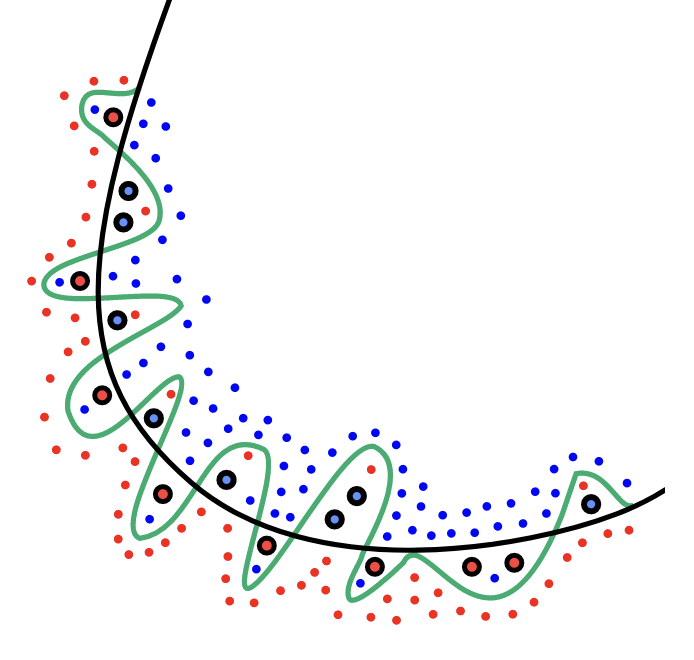
\includegraphics[width=0.3\textwidth]{images/overfitting.png}
    \caption{Example of overfitting}
\end{wrapfigure}

Care must be taken when selecting the function space to avoid overfitting\footnote{We say that the function \emph{overfits} the data when it corresponds too closely to the specific set of data (i.e. on the training data), such that it fails to fit additional data (i.e. test data).}: for example, if we were to choose $\mathcal{F}:=\R_d[X]$ for some $d\in\N$, it is in our best interest to keep $d$ small to avoid getting a function $f$ which fits perfectly the points but diverges between them. Although the empirical mean square error $\hat{R}_n$ decreases when the function space $\mathcal{F}$ becomes larger (i.e. larger polynomial degrees), the $\hatf_n$ estimator loses its predictive power. $\hatf_n$ will not necessarily perform well on new data. In what follows, we will consider the linear function space, containing functions of the form $f:x\mapsto ax+b$, which is the simplest.

\subsection{General setup and notations for supervised learning}
\begin{definition}[Training data set]
    The \emph{training data set}, often denoted $D_n:=\set{(x_i, y_i)}{i\in\llbracket 1, n \rrbracket}$, is the set of some observations $(x_i, y_i)\in\X\times\Y$. We will often make the assumption that the observations $(x_i, y_i)$ are realizations of i.i.d. random variables from a distribution $\nu$.
\end{definition}

The distribution $\nu$ is unknown to the statistician; it's a matter of learning it from the data.

\begin{definition}[Learning rule]
    A \emph{learning rule} $\A$ is a function that associates to training data $D_n$ a prediction function $\hatf_n$:
    \begin{equation*}
        \begin{aligned}
            \A: \bigcup_{n\in\N} (\X\times\Y)^n &\longrightarrow \Y^\X\\
            D_n &\longmapsto \hatf_n
        \end{aligned}
    \end{equation*}
    The estimated function $\hatf_n$ is constructed to predict a new output $y$ from a new input $x$, where $(x, y)$ is a pair of \emph{test data}, i.e. not necessarily observed in the training data. The function $\hatf_n$ is an estimator because it depends on the data $D_n$ and not on unobserved parameter, such as the distribution $\nu$. If $D_n$ is random, it is also a random function.
\end{definition}

\begin{definition}[Sqaured Loss Risk]
    Given an estimator $\hatf_n$, we define its risk:
    \begin{equation}
        \risk(\hatf_n) := \E\left[(Y-\hatf_n(X))^2\,\big| \, D_n\right] \quad \textnormal{where} \quad (X, Y)\sim\nu
    \end{equation}
\end{definition}

In practice, the statistician cannot compute the risk, since one cannot acces the distribution $\nu$. Therefore, a common method in supervised machine learning is to replace the risk (defined using the distribution $\nu$ through the expectation $\E$) by the empirical risk (defined using the training data set).

\begin{definition}[Squared Loss Empirical risk]
    Given an estimator $\hatf_n$ and a data set $D_n=\set{(x_i, y_i)}{i\in\iset{1}{n}}$, we define its \emph{empirical risk}:
    \begin{equation}
        \emrisk_n(f) := \frac{1}{n}\sum_{i=1}^n (y_i-f(x_i))^2
    \end{equation}
\end{definition}

\begin{wrapfigure}{r}{0.45\textwidth}
    \centering
    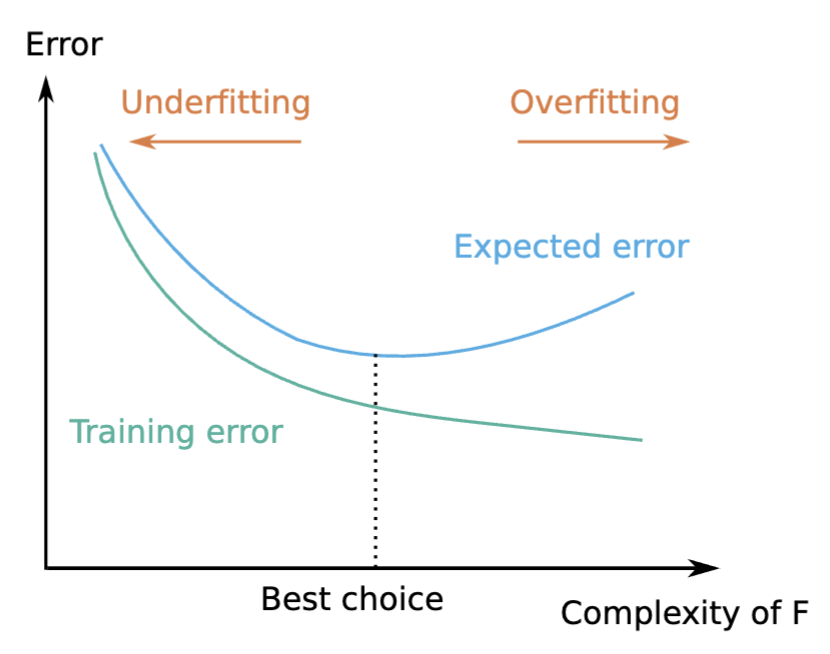
\includegraphics[width=0.4\textwidth]{images/learning-curves.png}
    \caption{Overfitting and underfitting according to the complexity of $\mathcal{F}$}
\end{wrapfigure}
However, one must be careful about overfitting, the case where $\emrisk_n(f)$ is much lower than $\risk(f)$, as discussed previously. In this chapter, we will study the performance of the least square estimator in the case of the linear model.

\begin{definition}[Linear model]
    When $\X=\R^d$ and $\Y=\R$, the simplest interesting function space is the set of affine functions. To ease the notation, we assume that the frist components of the inputs is 1 so that it is sufficient to consider linear functions. Therefore, the function space is:
    \begin{equation}
        \mathcal{F}:=\set{x\mapsto \theta^\top x}{\theta\in\R^d}
    \end{equation}
    i.e. linear functions parametrized by $\theta\in\R^d$.
\end{definition}

\begin{remark}
    Choosing a linear model, the empirical risk minimization corresponds to the problem of minimizing the following quantity over $\theta\in\R^d$:
    \begin{equation*}
        \emrisk_{\theta}:=\frac{1}{n}\sum_{i=1}^n(y_i-\theta^\top x_i)^2
    \end{equation*}
    This expression can be rewritten using matrix notation. We let $Y=(Y_1, \dots, Y_n)^\top\in\R^n$ be the vector of outputs and $X\in\R^{n\times d}$ the matrix of inputs, whose rows are $x_i^\top$. $X$ is called the \emph{design matrix}. The empirical risk is therefore given by:
    \begin{equation*}
        \emrisk_n(\theta)=\frac{1}{n}\norm{Y-X\theta}^2_2
    \end{equation*}
\end{remark}

\subsection{Ordinary Least Squares Estimator (OLS)}

\subsection{Statistical analysis}

\subsection{Ridge regression}

\section{Logic regression and convex analysis}
\subsection*{Recap of important notions and notations}
We are given an input space $X$ and an output space $Y$. We want to learn the relationship between input and output, modelised by a probability distribution $\rho\in \P(X\times Y)$. Thus, we try to find the best function $f_\star:X\to Y$, given a loss function $l:Y\times Y\to\R$. Therefore, $f_\star$ is often defined by:
\begin{equation*}
    f_\star = \argmin_{f:X\to Y} \E_{X, Y}[l(f(X), Y)]
\end{equation*}
where
\begin{equation*}
    \E_{X, Y}[g(X, Y)] = \int_{\R^2} g(x, y) \cdot \mathrm{d}\rho(x, y)
\end{equation*}

In practice, you only know some samples $D_N=[(x_1, y_1), \dots, (x_N, y_N)]$ with $(x_i, y_i) \sim \rho$, making it impossible to choose such an $f_\star$. Therefore, we try to find a good model $\hatf_{D_N}$, such that
\begin{equation*}
    \lim_{N\to+\infty}\mathcal{E}(\hatf_{D_N}) - \mathcal{E}(f) = 0
\end{equation*}
Such a result will often be given by a \emph{learning rate function} $c(N)$, with
\begin{equation*}
    \E_{D_N}[\mathcal{E}(\hatf_{D_N}) - \mathcal{E}(f)] \leq c(N) = o(1)
\end{equation*}
The function $\hatf_{D_N}$ can be chosen such that it minimizes the empirical error:
\begin{equation*}
    \hatf_{D_N} = \argmin_{f\in\mathcal{H}}\hat{\mathcal{E}}(f) = \argmin_{f\in\mathcal{H}} \frac{1}{N} \sum_{i=1}^N l(f(x_i), y_i)
\end{equation*}

\subsection{}
We consider the case where $X=\R^d$ and $Y=\R$. We define the loss $l$ to be the least squares, $l(y, y') = (y-y')^2$, and we choose our functions to be of the form of $f_\star = \theta_\star^T X$. In this case, ERM is OLS:
\begin{equation*}
    \hat{\theta}_N = \argmin_{\theta\in\R^d} \frac{1}{N} \sum_{i=1}^N (\theta^Tx_i-y_i)^2
\end{equation*}

We can also define $\hat{\theta}_{N, \lambda}$ to be:
\begin{equation*}
    \hat{\theta}_{N, \lambda} = \argmin_{\theta\in\R^d} \frac{1}{N} \sum_{i=1}^N (\theta^Tx_i-y_i)^2 + \lambda\norm{\theta}^2
\end{equation*}
This allows to regulate the "complexity" of the function to avoid overfitting. This is called Tikhonov regularization. In this case, we have
\begin{equation*}
    \E_{\hat{Y}}[\mathcal{\hat{\theta}_N} - \mathcal{E}(\theta_\star)] = \frac{\sigma^2 d}{N}
\end{equation*}
and therefore the optimal function is 
\begin{equation*}
    \hatf_{N, \lambda} = \argmin_{f\in\mathcal{H}} \hat{\mathcal{E}}(f) + \lambda R(f)
\end{equation*}

We define $X\in\R^{N\times d} := (x_1^T, \dots, x_N^T)$, and $\hat{Y}=(\hat{y}_1, \dots, \hat{y}_n)$. We this notation, we have
\begin{equation*}
    \hat{\theta}_{N, \lambda} = \frac{1}{N}||X\theta-\hat{Y}||^2 + \lambda||\theta||^2
\end{equation*}
Thus, we have
\begin{equation*}
    \begin{aligned}
        \nabla\mathcal{L}(\theta) := \frac{2}{N}X^TX\theta - 2\frac{X^T\hat{Y}}{N}+2\lambda\theta &= 0\\
        (\frac{X^TX}{N}+\lambda)\theta &= X^T\hat{Y}
    \end{aligned}
\end{equation*}
therefore,
\begin{equation*}
    \hat{\theta}_{N, \lambda} = \left(\frac{X^TX}{N}+\lambda I\right)^{-1}\frac{X^T\hat{Y}}{N} = \left(X^TX+\lambda N I\right)^{-1}X^T\hat{Y}
\end{equation*}
We introduce the singular value decomposition of $X$:
\begin{equation*}
    X = U\Sigma V^T
\end{equation*}
where $U^TU = UU^T = I_N$, $V^TV = VV^T=I_d$, and $\Sigma$ is diagonal with $\forall i, \,\Sigma_{i, i} \geq 0$.
In this case,
\begin{equation*}
\begin{aligned}
    X^TX + \lambda NI_d &= V\Sigma U^T U \Sigma V^T + \lambda N I_d\\
    &= V(\underbrace{\Sigma^2 + \lambda N I}_{\textnormal{invertible}}) V^T
\end{aligned}
\end{equation*}

\section{Convex analysis and convex optimization}
\subsection{Constrained optimization problems}

\subsection{Optimization algorithms for unconstrained convex optimization}
\subsubsection{Gradient Descent}

\subsubsection{Stochastic Gradient Descent}

\section{Kernels}
\subsection{Introduction to kernels}
In this course, we often focused on prediction methods which are \emph{linear}, that is, the input data are vectors and the prediction function is linear (e.g. $f(x)=w^\top x$ for $w\in\R^d$). In this situation with given data $(x_i, y_i)$, the vector $w$ can be obtained by minimizing
\begin{equation*}
    \hat{L}(w)=\frac{1}{n}\sum_{i=1}^n l(y_i, w^\top x_i) + \lambda \Omega(w)
\end{equation*}

Classical examples are logistic regression or least-squares regression. These methods look at first sight of limited practical significance, because input data may not be vectors, and relevant prediction functions may not be linear.

The goal of kernel methods is therefore to go beyond these limitations while keeping the good aspects. The underlying principle is to replace $x$ by a function $\phi(x)\in\R^d$, \emph{explicitly} or \emph{implicitly}, and consider linear predictions in $\Phi(x)$, i.e. $f(x)=w^\top \phi(x)$. We call $\phi(x)$ the \emph{feature} associated to $x$.

\begin{example}[Linear regression]
    In the case of linear regression, $\phi(x)=x$ for $x\in\R^d$. As expected, this gives us linear models:
    \begin{equation*}
        f(x)=w^\top x = \sum_{j=1}^d w_jx_j
    \end{equation*}
\end{example}

\begin{example}[Polynomial regression of degree $r$]
    With $x\in\R$, we have $\phi(x)\in\R^{r+1}$ defined by:
    \begin{equation*}
        \phi(x)=(1, x, x^2, \dots, x^r)
    \end{equation*}
    Therefore, the prediction functions will be general polynomials of degree at most $r$:
    \begin{equation*}
        f(x)=w^\top\phi(x)=\sum_{j=0}^r (\phi(x))_j = \sum_{j=1}^r w_jx^j
    \end{equation*}
\end{example}

\begin{example}[Polynomial multivariate regression of degree $r$]
    We consider $x\in\R^d$ and
    \begin{equation*}
        \phi(x)=(x_1^{\alpha_1}, \dots, x_d^{\alpha_d})
    \end{equation*}
    with $\sum_{i=1}^d \alpha_i=r$. In this situation, $p=\binom{d+r-1}{r}$ might be too big for an explicit representation to be feasible;
\end{example}

\begin{example}[Generic set of functions]
    Let $\varphi_1, \varphi_r : \R^d \to \R$ be a set of functions of interest (e.g. a subset of the Fourier basis); we define $\phi(x) = (\varphi_1(x), \dots, \varphi_r(x))$ to have:
    \begin{equation*}
        f(x)=w^\top \phi(x) = \sum_{j=1}^rw_j\varphi_j(x)
    \end{equation*}
\end{example}

\subsection{Representer theorem}
\subsubsection{Theorem statement}
Given a dataset $x_1, \dots, x_n$, we are able to compute the observed feature maps $\phi_(x_1), \dots, \phi(x_n)$. We can ask ourselves if there exists an easier representation for $w$ in terms of these observed feature maps, i.e. we want to know if it is possible to characterize the minimum $\hat{w}$ of:
\begin{equation*}
    \hat{L}(w) = \frac{1}{n}\sum_{i=1}^n l(y_i, w^\top\phi(x_i)) + \lambda w^\top w
\end{equation*}
in the form of $\hat{w} = \sum_{i=1}^n \alpha_i\phi(x_i)$, with $\alpha_i\in\R$. The following theorem guarantees such characterization under basic properties of $\hat{L}$.

\begin{theorem}[Representer theorem]
    Let $\phi:\X\to\R^d$. Let $(x_1, \dots, x_n)\in\X^n$ and assume that $\Psi:\R^{n+1}\to\R$ is strictly increasing with respect to the last variable. Then, the minimum of
    \begin{equation*}
        \hat{L}(w) := \Psi(w^\top\phi(x_1), \dots, w^\top\phi(x_n), w^\top w)
    \end{equation*}
    is obtained for
    \begin{equation*}
        w=\sum_{i=1}^n \alpha_i \phi(x_i)
    \end{equation*} for some $\alpha\in\R^n$.
\end{theorem}

\begin{proof}
    % TODO
\end{proof}

\begin{corollary}
    For $\lambda>0$, 
    \begin{equation*}
        \min_{w\in\R^d} \frac{1}{n} \sum_{i=1}^n l(y_i, w^\top\phi(x_i)) + \frac{\lambda}{2} w^\top w
    \end{equation*}
    is obtained for
    \begin{equation*}
        w = \sum_{i=1}^n \alpha_i\phi(x_i).
    \end{equation*}
\end{corollary}

Note that there is no assumption on $l$, and in particular, no convexity assumption. This result is extendable to Hilbert spaces (RKHS), as we will see in the next section.

\subsubsection{Finite dimensional representation of the learning problem}
Using the representer theorem, we know that the minimum of $\hat{L}$ is of the form $w=\sum_{i=1}^n \alpha_i\phi(x_i)$; we can therefore directly optimize this characterization, i.e. we can then write:
\begin{equation*}
    \min_{w\in\R^r} \frac{1}{n} \sum_{i=1}^n l(y_i, w^\top\phi(x_i)) + \frac{\lambda}{2} w^\top w = \min_{\alpha\in\R^n} \frac{1}{n}\sum_{i=1}^n l(y_i, (K\alpha)_i) + \frac{\lambda}{2}\alpha^\top K\alpha
\end{equation*}
where $K$ is an $n\times n$ matrix with values
\begin{equation*}
    K_{i, j} = \phi(x_i)^\top \phi(x_j).
\end{equation*}

Indeed,
\begin{equation*}
    \phi(x_i)^\top w = \sum_{j=1}^n \alpha_j\phi(x_i)^\top\phi(x_j) = (K\alpha)_i
\end{equation*}
moreover,
\begin{equation*}
    ||w||^2 = w^\top w = \sum_{i=1}^n\sum_{j=1}^n \alpha_i\alpha_j\phi(x_i)^\top\phi(x_j) = \alpha^\top K\alpha
\end{equation*}

We finally have a closed form representation for the function evaluation. Defining the \emph{kernel function} $k(x, x'):=\phi(x)^\top \phi(x')$, we have:
\begin{equation*}
    f(x) = w^\top\phi(x) = \sum_{i=1}^n \alpha_i\phi(x_i)^\top\phi(x) = \sum_{i=1}^n \alpha_i k(x_i, x).
\end{equation*}

\begin{remark}[Kernel trick]
    The whole learning problem can be written in terms of the kernel $k$; indeed, $f$ depends only on $k$, $\hat{L}$ depends on $K$ with $K_{i, j} = k(x_i, x_j)$. Therefore, we have the so-called \emph{kernel trick}, i.e. we do not need to compute explicitly the features $\phi$ to be able to represent and solve the learning problem, we just need to be able to compute their inner product.
\end{remark}

\begin{example}[Power of the kernel trick with infinite dimensional feature maps]
    \leavevmode
    
    \noindent
    Consider $\X=\lbrack-1, 1\rbrack$ and the feature map
    \begin{equation*}
        \phi(x)=(1, x, x^2, \dots).
    \end{equation*}
    The resulting model space would have the form
    \begin{equation*}
        f(x)=\sum_{j=0}^{+\infty}w_jx^j
    \end{equation*}
    with $\sum_{j=1}^{+\infty}w_j^2 < +\infty$. This model space is the set of analytic function on $\X$, which is a very rich space. In particular, it is dense in the space of continuous functions. However, it is not possible to compute $\phi(x)$ explicitly since it is infinite dimensional. The kernel trick provides an elegant way to compute the solution of the learning problem in closed form; indeed, the inner product can be computed in closed form in $O(1)$:
    \begin{equation*}
        k(x, x') = \phi(x)^\top\phi(x')=\sum_{j=0}^{+\infty}x^jx^{'j} = \frac{1}{1-xx'}
    \end{equation*}

    Therefore, the kernel trick allow to replace $\R^d$ by $\R^n$, which is interesting when $d$ is very large. Furthermore, it allows to separate the representation problem (design a kernel on a set $\X$), algorithms, and analysis (which only use the kernel matrix $K$).
\end{example}

\subsection{Properties of kernels}
Since the learning problem is completely defined in terms of the kernel function, the explicit knowledge of the feature map is not required anymore. In particular, given a function $k:X\times X \to \R$, tu use it in a learning problem, we need to be sure that it is a \emph{positive definite kernel}, i.e. that there exists a feature map $\phi$ such that
\begin{equation*}
    \forall x, x'\in\X, \quad k(x, x") = \phi(x)^\top \phi(x')
\end{equation*}
Kernel functions admits many characterizations, which we will now present.

\begin{property}[Characterization in terms of positive-definitness]
    $k$ is a positive definite kernel if and only if the kernel matrix $k$ is positive semi-definite (i.e. all its eigenvalues are non-negative).
\end{property}

\begin{theorem}[Aronsazjn]
    $k$ is a positive definite kernel if and only if there exists a Hilbert space $\mathcal{F}$, and $\phi:X\to\mathcal{F}$ such that
    \begin{equation*}
        \forall x, y\in X, \quad k(x, y) = \trace{\phi(x), \phi(y)}
    \end{equation*}
    If such objects exist, $\mathcal{F}$ is called the \emph{feature space} and $\phi$ the \emph{feature map}.
\end{theorem}

\begin{property}
    The sum and product of kernels are kernels.
\end{property}

\begin{example}[Linear kernel]
    The linear kernel corresponds to $\phi = x \mapsto x$:
    \begin{equation*}
        k(x, y) = x^\top y
    \end{equation*}
\end{example}

\begin{example}[Polynomial kernel]
    The kernel $k(x, y) = (x^\top y)^r$ can be expanded as:
    \begin{equation*}
        k(x, y) = \left(\sum_{i=1}^d x_iy_i\right)^r = \sum_{\alpha_1 + \dots + \alpha_p=r} \binom{r}{\alpha_1, \dots, \alpha_p} \underbrace{(x_1y_1)^{\alpha_1} \dots (x_py_p)^{\alpha_p}}_{(x_1^{\alpha_1}\dots x_p^{\alpha_p})(y_1^{\alpha_1}\dots y_p^{\alpha_p})}
    \end{equation*}
\end{example}

\begin{example}[Translation-invariant kernels on a bounded interval]
\end{example}

\begin{example}[Translation-invariant kernels on $\R^d$]
\end{example}

\section{Elements of Statistical Machine Learning}

\section{Model-Based Machine Learning}

\section{Maximum Likelihood}

\section{Unsupervised Learning}

\section{MCMC Sampling}

\section{Neural Networks}

\end{document}